\section{Breakoutboards} \label{sec:breakoutboards}

Da AutoGreen er tiltænkt at skulle monitorere temperatur, luftfugtighed og lysintensitet, blev der valgt nogle sensorer der kunne foretage målinger af disse variable. 

Temperatur- og luftfugtighedssensoren som blev valgt var en \textit{HONEYWELL S\&C  HIH6030-021-001} \cite{lib:TempHum_DS}. Sensoren følger en standard \IIC-protokol og det er nødvendigt at tage hensyn til \IIC-klokkens hastighed samt spændingen på \IIC-bussen, så det er muligt for alle enheder på bussen at kommunikere. Fra producenten har sensoren fået en standard adresse, som skal bruges til kommunikation med enheden.

Lyssensoren der blev valgt var en \textit{Intersil ISL29010IROZ}\cite{lib:LightSens}. Lysfølsomheden kan ændres i sensoren ved at ændre en reference vha. forskellige modstandsstørrelser. Intensiteten af lyset måles i lumen, og sensoren kan måle fra 0 til 128.000 lumen, hvilket passer fint til drivhuset, som kan stå både i mørke og i stærk sollys. Som udgangspunkt oplyser databladet at sensoren fungerer bedst som vist i multisimdiagrammet i Figur \ref{fig:temp_fugt_lys_design}.

Størrelsen på sensorene gør dem meget svære at arbejde med, så der blev designet et breakoutboard til hver sensor. 
Både Temp/Luftfugt og Lyssensoren er af SOIC typen og meget små, så der er anvendt Multisim og Ultiboard til design af breakoutboards, så interfacing med sensorerne blev gjort væsentligt nemmere. Kredsløbene for breakout boards kan ses i Figur \ref{fig:temp_fugt_lys_design}. 

\begin{figure}[h]
\centering
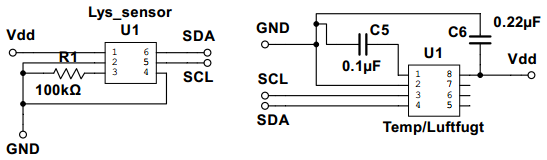
\includegraphics[trim=0 0 0 0, clip=true]{../fig/TempOgLys.png}
\caption{Design af temp/luftfugtsensor og lyssensor breakoutboards.}
\label{fig:temp_fugt_lys_design}
\end{figure}

Alle komponenters værdier fra billederne er taget fra sensorernes datablade.

\clearpage